\documentclass[times, utf8, zavrsni]{fer}
\usepackage{booktabs}
\usepackage{listings}
\usepackage[toc,page]{appendix}

% JavaScript
\lstdefinelanguage{JavaScript}{
  morekeywords={typeof, new, true, false, catch, function, return, null, catch, switch, var, if, in, while, do, else, case, break, class, let, import, @, export},
  morecomment=[s]{/*}{*/},
  morecomment=[l]//,
  morestring=[b]",
  morestring=[b]'
}

% PureScript
\lstdefinelanguage{PureScript}{
  morekeywords={module, where, import, Int, String, foreign, Number},
  morecomment=[s]{/*}{*/},
  morecomment=[l]--,
  morestring=[b]",
  morestring=[b]'
}

\lstset{
	lineskip={-1.3pt},
    frame=single,
    breaklines=true
}

\begin{document}

\newcounter{MyBibCount}
\makeatletter
\renewcommand{\@biblabel}[1]{\stepcounter{MyBibCount}\theMyBibCount.}
\makeatother

\nocite{*}

% TODO: Navedite broj rada.
\thesisnumber{4749}

% TODO: Navedite naslov rada.
\title{Funkcijski pristup razvoju Web korisničkih sučelja}

% TODO: Navedite vaše ime i prezime.
\author{Dominik Ivošević}	

\maketitle

% Ispis stranice s napomenom o umetanju izvornika rada. Uklonite naredbu \izvornik ako želite izbaciti tu stranicu.
\izvornik

% Dodavanje zahvale ili prazne stranice. Ako ne želite dodati zahvalu, naredbu ostavite radi prazne stranice.
\zahvala{Zahvaljujem svojem mentoru profesoru Vladi Sruku na pomoći i savjetima te svojoj sestri Mihaeli, roditeljima i djevojci Ani na podršci u teškim vremenima}

\tableofcontents

\chapter{Uvod}
Već neko vrijeme se može primijetiti trend razvoja sve većih sustava na web platformi. U današnje doba je veoma bitno da  aplikacija može što prije doći do korisnika i to u što manje koraka na što više operativnih sustava u isto vrijeme. Kad danas čovjek radi nešto za računalom i kad mu stigne poruka mu u isto vrijeme zvoni laptop, mobitel, tablet i sat. Kako bi se mogao razvijati isti sustav za što više platformi u isto vrijeme vrlo je bitno da se što prije prestane pisati zasebni kod za svaki sustav posebno. Također je bitno da takav kod ima karakteristike pouzdanosti, jednoznačnosti, ekspresivnosti i efikasnosti.

Kao vrlo zanimljiva kombinacija se pokazuje razvoj web sustava u statičkom funkcijskom jeziku.

U počecima interneta se većina razvoja odvijala na poslužiteljskoj strani (eng. back end) koji je slao gotove predloške (eng. template) pregledniku i koji je zatim to prikazao. S vremenom su se pokazale potrebe za nekim sitnim funkcionalnostima za koje bi bilo praktično da se ne mora osvježiti stranica. Tu se pojavio JavaScript, jezik koji nikad nije predviđen za razvoj ozbiljnih sustava, ali je odlično obavljao manje zadatke u par linija koda. Kako je web napredovao tako su se počele pokazivati potrebe za sve više i više funkcionalnosti. Stranice koje se ne osvježavaju, modeli i poslovna logika se obrađuju na klijentskoj strani, stranice komuniciraju s poslužiteljem samo da dohvate datoteke i pošalju upit na bazu.

U takvim uvjetima se dinamički jezik pokazuje kao loš izbor. Kako bi se izbjegle neplanirane greške pri manipulaciji s modelima tijekom provođenja poslovne logike potreban je jezik koji pazi da se ne ostane bez podataka i da se ne bi slučajno izvodile neplanirane operacije. Bilo bi interesantno proučiti kako će se funkcijski jezik snalaziti u okruženju s tradicionalno puno mutacija makar se nepromjenjive (eng. immutable) strukture sve ozbiljnije uzimaju u obzir kod modeliranja pomoćnih biblioteka i u jezicima koji podržavaju mutacije. Također su se funkcijski jezici pokazali vrlo prikladni za testiranje zbog načina na koji se piše kod koji se može u konačnici zamisliti kao cjevovod (eng. pipeline) koji se može na dva dijela izolirati i onda se može "testirati propusnost".

U ovom radu primarni je cilj proučiti spoj biblioteke za razvoj korisničkih sučelja Angular 2 koji je pisan u jeziku  TypeScript i statičkog funkcijskog jezika PureScript koji je vrlo inspiriran Haskellom.

U prvoj cjelini će se proučavati tehnologije kojima će se baratati. Proučit će se novi standard web komponenata, oblikovni obrazac model-pogled-model pogleda i jezike TypeScript i PureScript i način na koji se oni prevode u JavaScript.

U drugoj cjelini će se proučavati problem prijenosa biblioteke Angular 2 iz jezika TypeScript u jezik PureScript te će se na tom primjeru proučavati generalni problemi oko prijenosa biblioteke iz objektno orijentiranog ekosustava u funkcijski deklarativni ekosustav.

\chapter{Funkcijski Web}
Budući da su tehnički zahtjevi za pokretanje internetskog preglednika postali toliko mali da si skoro svatko može priuštiti pristup internetu, logičan korak za dohvaćanje što većeg broja korisnika je razvoj web aplikacija. JavaScript je danas temeljni jezik za bilo kakvo izvođenje koda u pregledniku, ali kad je on nastajao nitko nije zamišljao u kojim će se sve oblicima koristiti. Kako se povećavalo područje u kojem se jezik koristio, tako su se krenuli i povećavati zahtjevi za sam jezik. Trenutno se jezik nalazi u verziji koja se naziva ECMAScript 5 te je 2016. godine dovršena specifikacija ECMAScript 6 i razvojni timovi preglednika su već započeli s implementacijom tog standarda (a i nekih karakteristika ECMAScript 7 koji je tek u začecima). Kako raste popularnost JavaScripta i širi područje primjene tako nastaju dijalekti jezika koji pokušavaju poboljšati jezik dalje od njegove specifikacije kako bi se lakše prilagodio području primjene i zahtjevima koji dolaze s njim. 

Jedan od popularnijih dijalekata je CoffeScript koji je nastao 2009. godine i inspiriran je jezicima Ruby, Python i Haskell. 2012. godine pod pokroviteljstvom Microsofta kreće razvoj jezika  koji je također dijalekt JavaScripta koji pokušava naglasiti razvoj na objektno orijentiranom principu dodajući tipove i klase. Kako se povećala kvaliteta alata za implementiranje svojih dijalekata JavaScripta koji se prevode u njega tako se počelo viđati sve zanimljivije varijante sa svojim karakteristika i prednostima (a i manama).

Još jedan zanimljiv trend koji se može vidjeti je primjena raznih tehnika na razvoj aplikacija u JavaScriptu. Sve je veći naglasak na komponentiziranju, tipiziranju, uklanjanju sporednih efekata itd. Za razvoj velikih web aplikacije koje imaju velik niz funkcionalnosti potrebna je disciplina, opreznost i strukturiranost te se sve više poseže za ekspresivnijim jezicima.

Svaki jezik ima tendenciju ponuditi svoje preporučene implementacije nekih često korištenih programskih oblikovnih obrazaca kao MCV, MVVM, reaktivno programiranje i slično. Knockout.js, React.js i Angular.js su danas najpopularnije biblioteke za razvoj korisničkih sučelja u JavaScriptu, Angular 2 je za rad u TypeScriptu, a PureScript Halogen je najpopularniji za rad u PureScriptu uz biblioteke kao što su PureScript React i PureScript Thermite koji omogućavaju korištenje React biblioteke unutar PureScript ekosustava.

Postoje još biblioteke kao ReactiveX koje imaju implementacije u mnogim jezicima pa tako i Javascriptu/TypeScriptu/PureScriptu koje pružaju jednostavno sučelje za izgradnju sustava koristeći funkcijski pristup i oblikovne obrasce nadgledatelj i iterator te se takve datoteke često koriste kao pomoćne datoteke u sklopu većih biblioteka (ReactiveX je integralni dio Angular 2 načina).

\section{Web sučelja i biblioteke}
Jedna od najpopularnijih biblioteka korisničkih sučelja danas je Angular. Ona pokušava pojednostaviti razvoj web sučelja tako što pruža razne funkcionalnosti kao preusmjeravanje, predlošci i testiranje. Također postavljajući neke generalne smjernice za razvoj koda omogućava izgradnju vrlo kvalitetnih, fleksibilnih, efikasnih i pouzdanih web sučelja. Vrlo interesantan aspekt biblioteke Angular 2 je da se vrlo usko integrira uz neke od drugih biblioteka i tehnologija koje su u velikom zamahu te se tako stvara ekosustav profesionalnih alata otvorenog koda. Također, Angular 2 radi vrlo blisko uz Web standard Web komponenata koji pruža dodatne prednosti.

\section{Web komponente}
Web komponente su niz standarda koji se razvijaju kako bi se omogućilo razvijanje ponovno iskoristivih komponenata unutar web dokumenata i aplikacija. Cilj je omogućiti razvoj temeljen na komponentama na WWW-u. Model komponenata omogućava enkapsulaciju i međusobnu izmjenjivost zasebnih HTML elemenata.
Web komponente se sastoje od 4 glavna elementa koji se mogu koristiti odvojeno ili skupa:
umjetni elementi, Shadow DOM, HTML Imports i HTML Templates.

\subsection{Deklarativni sjenoviti DOM}
Sjenoviti DOM [5] omogućava enkapsulaciju JavaScripta, CSS-a i izradu predložaka za neku Web komponentu. Sjenoviti DOM omogućava da ove stvari ostanu odvojene od DOM-a ostatka dokumenta. Sjenoviti DOM se također može koristiti izvan Web komponente.

Jedan od razloga zašto bi se želio koristiti dio koda odvojen od ostatka stranice je na primjer kod razvoja velikih web stranica. Vrlo često je teško odražavati jedinstven i konzistentan CSS kroz cijelu stranicu pa se zna dogoditi da stil od navigacijske komponente procuri u ostatak stranice i slično. Kako stranica raste sve je teže ovakve stvari kontrolirati i alat kao sjenoviti DOM omogućava imati jasne granice.

Sjenoviti DOM mora uvijek biti pričvršćen za postojeći element. Element može biti postojeći element u HTML datoteci ili element stvoren u DOM-u skriptiranjem. Može biti nativni element ili neki novi. Stvara se pozivom na elementu Element.createShadowRoot() kao u primjeru:

\begin{lstlisting}[language=HTML, basicstyle=\small\linespread{0.8}]
<html>
  <head></head>
  <body>
    <p id="hostElement"></p>
    <script>
      // Stvaranje sjenovitog DOM-a na elementu <p>
      var shadow = document.querySelector('#hostElement').createShadowRoot();
    </script>
  </body>
</html>
\end{lstlisting}

Također se može dodati izolirani CSS kao u sljedećem primjeru koji boja sjenoviti DOM tekst u crveno:

\begin{lstlisting}[language=HTML, basicstyle=\small\linespread{0.8}]
<script>
  // Stvaranje sjenovitog DOM-a
  var shadow = document.querySelector('#hostElement').createShadowRoot();
  // Dodavanje teksta na sjenoviti DOM
  shadow.innerHTML = '<p>Here is some new text</p>';
  // Dodavanje CSS-a kako bi tekst bio crven
  shadow.innerHTML += '<style>p { color: red; }</style>';
</script>
\end{lstlisting}

\subsection{Umjetni elementi}
Umjetni elementi [4] (eng. Custom Elements) su također dio razvijanog standarda Web komponenata. Umjetni elementi omogućavaju stvaranje vlastitih HTML znački i elemenata koji mogu imati svoje skriptirano ponašanje i CSS stil.

Na prvi pogled se ne čini toliko korisnim budući da se moglo i prije napraviti umjetni element i ručno ga stilizirati i skriptirati ponašanje. Ono što je posebno kod umjetnih elemenata je da se može koristiti povratne pozive životnog vijeka (eng. lifecycle callbacks) koji omogućuju da dodajemo ponašanje na određene dijelove životnog vijeka elementa. Na primjer se može dodati određeno ponašanje elementu kada se on dodadje u DOM, a drugo kad ga se uklanja.

Dijelovi životnog vijeka:
\begin{itemize}
\item createdCallback - ponašanje kad se element registrira
\item attachedCallback - ponašanje kad se element umeće
\item detachedCallback - ponašanje kad se element uklanja
\item attributeChangedCallback - ponašanje kad se ažurira atribut elementa
\end{itemize}

\section{Obrazac model-pogled-model pogleda}
MPPM (eng. MVVM) je oblikovni obrazac koji omogućuje jasno i čisto odvajanje korisničkog sučelja i njegove logike. 
Postoje 3 osnovna dijela MPPM obrasca: model, pogled i model pogleda. Svaki obavlja posebnu i odvojenu ulogu unutar obrasca. Slika pokazuje Odnos između komponenata.

Prednosti MPPM-a:
\begin{itemize}
\item Tijekom razvojnog procesa, programeri i dizajneri mogu odvojeno i zajedno raditi na svojim komponentama. Dizajneri se mogu koncentrirati na pogled dok se programeri mogu skoncentrirati na poglede modela i modele.
\item Programeri mogu napraviti testove za model pogleda i model bez da koriste pogled. Jedinični testovi za model pogleda mogu identično oponašati funkcionalnost pogleda.
\item U slučaju da već postoji model u kojem se nalazi poslovna logika koja je presložena da bi se ponovno implementirala onda model pogleda se može ponašati kao prilagođivač (eng. adapter) za uporabu tog modela u pogledu.
\end{itemize}


Komponente su odvojene jedne od drugih i to omogućava:
\begin{itemize}
\item Komponente mogu biti zamijenjene
\item Interna implementacija može biti izmijenjena bez da se razlika odražava na ostatak sustava
\item Svaka komponenta se može zasebno razvijati i zatim dodati u veću cjelinu 
\item Može se i zasebno testirati s jediničnim testovima (eng. unit tests)
\end{itemize}

Uz razumijevanje svakog od 3 dijela MPPM obrasca nužno je i biti upoznat s time kako se ti dijelovi odnose jedni na druge. Na "najvišoj razini", pogled "zna" za model pogleda, a model pogleda zna za model, ali model nije svjestan postojanja pogleda modela i model pogleda nije svjestan postojanja pogleda. Model pogleda izolira pogled od klasa modela i omogućava modelu da se razvija neovisno o pogledu.

\subsection{Pogled}
Pogled je odgovoran za definiranje strukture, izgleda i dojma onog što korisnik vidi na ekranu. Idealno, pogled je definiran s što više HTML-a i što manje bilo kakve logike u obliku skripti koje nikako ne sadrže poslovnu logiku.

\subsection{Model}
Model u obrascu MPPM je implementacija aplikacijskog domenskog modela koji uključuje podatkovni model i poslovnu i validacijsku logiku. Primjeri modela su spremnici (eng. repository), poslovni objekti, objekti za prijenos podataka (eng. data transfer objects) ili vrlo jednostavnih objekata (eng. POCO) ili nešto drugo.

\subsection{Model pogleda}
Model pogleda se ponaša kao medijator između pogleda i modela i odgovoran je za procesiranje logike pogleda. Uobičajeno je da tijekom interakcije model pogleda poziva metode koje se nalaze na klasama modela. Zatim model pogleda pruža informacije koje je dobio od modela pogledu tako da ih on može jednostavno prikazati te može dodatno obraditi te podatke kako bi bili čitljiviji i jasniji. 
Model pogleda također pruža implementacije komandi koje korisnik aplikacije može pozvati iniciranjem akcije. Također je model pogleda odgovoran za pohranjivanje i menadžeriranje stanja u kojima se nalazi pogled (na primjer ako je stisnut gumb za brisanje nečega i trenutno je faza zahtjeva potvrde ili ako je započeto povlačenje nekog elementa, ali još nije "bačen".

\subsection{Spajanje pogleda modela i pogleda}
Postoje mnogi pristupi spajanju pogleda modela i pogleda uključujući direktno povezivanje i spremnički pristup. Međutim, svi pristupi dijele isti konačni cilj.

\subsection{Obrazac model-pogled-kontroler opisan u kontekstu Angular 2}
MPPM i MPK su dva obrasca koji dijele mnogo zajedničkih karakteristika i makar mnogi nazivaju Angular 2 [1] tipičnim primjerom MPPM obrasca, razvojni inženjeri Angular-a su odlučili opisati Angular 2 u kontekstu MPK obrasca pa proučavamo kako su oni zamislili.
Angular aplikacija se sastoji od korijenske komponente koja može sadržavati ostale komponente tvoreći stablo komponenata. Vezivanje podataka (eng. data binding) omogućava automatsko prosljeđivanje podataka iz roditeljske u dječju komponentu. Komande omogućavaju roditelju zahtjevanje nusprodukata od komponente djeteta. Događaji omogućuju komponenti djeteta da obavijesti roditelja o promjeni stanja. 

Promatramo izvedbu MVP(eng. MVC) principa na primjeru u biblioteci Angular 2:

\subsubsection{Komponenta}
Komponente su osnovni gradivni blokovi web aplikacija. Oni se sastoje od kontrolera, pogleda i detektora. Kontroler određuje karakteristike komponente. Povezuje ju sa svojim templateom, stilovima, određuje karakteristično ime na koje će se vezati u DOM-u i drugo.

\subsubsection{Pogled}
Pogled je vizualna reprezentacija sučelja. Jedan pogled se može sastojati od drugih komponenata ili HTML primitiva. Postavljanje propertyja na pogledu osvježuje dječju komponentu ili property od HTML elementa. Okidanjem akcije na pogledu pokreće metodu na dječjoj komponenti ili na HTML elementu. Pogled može slušati dječju komponentu ili HTML elemente i zatim pozivati metode na kontroleru.

\subsubsection{Model}
Modeli su definirano preko tipova te se pohranjuju unutar kontrolera koji se veže s pogledom na kojem onda korisnik može vidjeti te podatke.

\section{Web jezici}
Jedan od glavnih ciljeva je proučiti karakteristike jezika u čijim će se ekosustavima raditi te razmotriti na koji način će se omogućiti pisanje poziva Angular 2 koda u ekosustavu jezika PureScript. Prvi korak je proučiti svaki jezik zasebno, a nakon toga je cilj proučiti kako da kod pisan u jeziku PureScript ima pristup smislenom API-ju koji reprezentira filozofiju Angular 2 biblioteke, tzv. "Angular način" (eng. "The Angular Way"). Ono što veoma brzo postane očito pri pokušaju ostvarivanja ovog cilja je da se jezici TypeScript i PureScript veoma razlikuju makar prevedeni kod od oba jezika postaje ispravan JavaScript kod. 

Kako bi uspješno omogućili korištenje Angular 2 biblioteke u PureScriptu, proučit će se specijalizirane alate PureScripta koji služe baš tome da se jedan deklarativni funkcijski jezik uspješno prevede u imperativni "objektno orijentirani" jezik. Razlog zbog čega je prethodno "objektno orijentirani" stavljeno pod navodnike je jer makar JavaScript sam po sebi nije klasični objektno orijentirani jezik, TypeScript koji je predviđen za pisanje koda koji je najkompatibilniji s Angular 2 bibliotekom ima veoma široko korištenje objektno orijentiranih oblikovnih obrazaca te makar u prevedenom kodu nema takvih konstrukata, TypeScript kod ima široku uporabu raznih objektno orijentiranih konstrukata kao klase, dekoratori, konstruktori, kontekst klase, pripadne funkcije klase te makar je Angular 2 pisan s velikim naglaskom na deklarativni opis komponenata i dalje se u radu u TypeScriptu pojavljuju iterativna rješenja nekih problema koja će se morati u PureScriptu preoblikovati i prilagoditi funkcijskom pristupu.

\section{TypeScript}
Typescript je trenutno najbrže rastući jezik po popularnosti od svih JavaScript dijalekata. To je opcionalno tipiziran jezik baziran na klasnom objektno orijentiranom pristupu. Gospodin Anders Hejlsberg, glavni arhitekt C\#-a i kreator jezika Delphi i Turbo Pascal je radio na razvoju TypeScripta. TypeScript je osmišljen za uporabu u razvoju velikih aplikacija i transprevodi (eng. transpiles) se u JavaScript. Budući da je TypeScript nadskup JavaScripta, svaki postojeći JavaScript kod je ispravan TypeScript kod. To igra ogromnu ulogu u omogućavanju prelaska starijih baza koda na TypeScript. TypeScript omogućava definicijske datoteke koje sadrže podatke o tipovima postojećih JavaScript biblioteka kako bi se što bezbolnije mogao JavaScript kod tipizirati i integrirati u neki TypeScript ekosustav. To je nalik tome da C/C++ glavne (eng. header) datoteke mogu opisivati strukturu postojećih objektnih datoteka.

\subsection{Ciljevi}
\begin{itemize}
\item Statički identificirati konstrukte koji su vjerojatno pogreška.
\item Omogućiti strukurni mehanizam za velike količine koda.
\item Ne smije stvarati nikakav dodatan trošak na izvršavanje prevedenog koda.
\item Rezultantni prevedeni kod mora biti čitljiv i shvatljiv.
\item Mora pratiti trenutne i buduće ECMAScript specifikacije.
\item Mora koristiti konzistentan i izbrisiv strukturni sustav tipiziranja.
\item Mora biti izvodiv na više popularnih platformi.
\item Ne smije doći do bilo kakvih znatnih kritičnih promjena nakon verzije 1.0
\end{itemize}

\subsection{Tipovi i identifikatori u TypeScriptu}
U TypeScriptu postoje osnovni tipovi kakve viđamo i u ostalim jezicima.
\begin{itemize}
\item Bool vrijednost: let isDone: boolean = false;
\item Decimalni: let decimal: number = 0xf00d;
\item Heksadecimalni: let hex: number = 0b1010;
\item Oktalni: let octal: number = 0o744;
\item Nit: let color:string = "blue";
\item Niz: let list: Array<Number> = [1, 2, 3];
\item Par: let x: [string, number] = ["hello", 10];
\item Objekt: let o: { a: string, b: number } = { a: "qwe", b: 2 };
\end{itemize}

Za daljnji razvoj PureScript Angular 2 biblioteke je veoma bitno proučiti sličnosti i razlike između početnog TypeScripta rezultantnog JavaScripta te proučiti kako izgledaju neki jezični konstrukti kao klase iz TypeScripta kad se prevedu u JavaScript. Promatramo na primjeru jedne Angular 2 komponente. Ona omogućava pregledavanje postojećih zvučnih zapisa i ažuriranje informacija o njima.

\begin{lstlisting}[language=JavaScript, basicstyle=\small\linespread{0.8}]

// Uvodenje koristenih vanjskih biblioteka
import { Component } from 'angular2/core';
import { Location, RouteConfig, RouterLink, Router, CanActivate } from 'angular2/router';
import { NgIf, NgFor, FORM_DIRECTIVES} from 'angular2/common';
import { HttpAdvanced } from '../../services/services';

// Dekoriranje klase
@Component({
    selector: 'ManageTracks',
    templateUrl: './dist/views/manageTracks/manageTracks.html',
    directives: [ NgFor, RouterLink ]
})
export class ManageTracks {
	// Deklaracija dosega klase
    http: HttpAdvanced;
    router: Router;

    tracks: Track[];
    editable: boolean = false;

	// Pripadne metode klase
    toggleEditable(){
        this.editable = !this.editable;
    }

    editTrack(track) {
        this.router.navigate(['EditTrack', { trackId: track.id }]);
    }

    deleteTrack(track) {
        for (let i in this.tracks) {
            let ii = parseInt(i);
            if (this.tracks[ii].id == track.id) {
                this.tracks.splice(ii, 1);
                break;
            }
        }
        this.http.postWithBothMsg('admin/tracks/' + track.id + '/delete', '');
    }
	
    // Deklaracija konstruktora klase
    constructor(router: Router, http: HttpAdvanced) {
        this.http = http;
        this.router = router;

        this.http.get('/tracks/list', (res) => {
            console.log(res);
            this.tracks = new Array();
            for (let i in res) {
                this.tracks.push(new Track(res[i]));
            }
        });
    }
}

// Definicija zasebnog pomocnog objekta
class Track {
    id: number;
    title: string;
    duration: number;
    artist: string;
    year: number;
    genre: string;

    constructor(values) {
        this.id = values.id;
        this.title = values.title;
        this.duration = values.duration;
        this.artist = values.artist;
        this.year = values.year;
        this.genre = values.genre;
    }
}

\end{lstlisting}


Rezultantni JavaScript kod je:

\begin{lstlisting}[language=JavaScript, basicstyle=\small\linespread{0.8}]

"use strict";
// Deklaracija funkcija koje se koriste kao prilagodnici za funkcionalnosti dekoriranja i pohrane metapodataka
var __decorate = (this && this.__decorate) || function (decorators, target, key, desc) {
    var c = arguments.length, r = c < 3 ? target : desc === null ? desc = Object.getOwnPropertyDescriptor(target, key) : desc, d;
    if (typeof Reflect === "object" && typeof Reflect.decorate === "function") r = Reflect.decorate(decorators, target, key, desc);
    else for (var i = decorators.length - 1; i >= 0; i--) if (d = decorators[i]) r = (c < 3 ? d(r) : c > 3 ? d(target, key, r) : d(target, key)) || r;
    return c > 3 && r && Object.defineProperty(target, key, r), r;
};
var __metadata = (this && this.__metadata) || function (k, v) {
    if (typeof Reflect === "object" && typeof Reflect.metadata === "function") return Reflect.metadata(k, v);
};
var core_1 = require('angular2/core');
var router_1 = require('angular2/router');
var common_1 = require('angular2/common');
var services_1 = require('../../services/services');
var ManageTracks = (function () {
    function ManageTracks(router, http) {
    	// Deklariranje dosega od funkcije
        // Izvrsavanje konstruktora
        var _this = this;
        this.editable = false;
        this.http = http;
        this.router = router;
        this.http.get('/tracks/list', function (res) {
            console.log(res);
            _this.tracks = new Array();
            for (var i in res) {
                _this.tracks.push(new Track(res[i]));
            }
        });
    }
    // Dodavanje funkcija na prototip
    ManageTracks.prototype.toggleEditable = function () {
        this.editable = !this.editable;
    };
    ManageTracks.prototype.editTrack = function (track) {
        this.router.navigate(['EditTrack', { trackId: track.id }]);
    };
    ManageTracks.prototype.deleteTrack = function (track) {
        for (var i in this.tracks) {
            var ii = parseInt(i);
            if (this.tracks[ii].id == track.id) {
                this.tracks.splice(ii, 1);
                break;
            }
        }
        this.http.postWithBothMsg('admin/tracks/' + track.id + '/delete', '');
    };
    // Dekoriranje funkcije s komponentom
    ManageTracks = __decorate([
        core_1.Component({
            selector: 'ManageTracks',
            templateUrl: './dist/views/manageTracks/manageTracks.html',
            directives: [common_1.NgFor, router_1.RouterLink]
        }), 
        // Pohranjivanje metapodataka za injektor ovisnosti
        __metadata('design:paramtypes', [router_1.Router, services_1.HttpAdvanced])
    ], ManageTracks);
    return ManageTracks;
}());

// Dodavanje objekta ManageTracks u objekt koji se izvozi iz modula
exports.ManageTracks = ManageTracks;

// Definicija zasebnog pomocnog objekta
var Track = (function () {
    function Track(values) {
        this.id = values.id;
        this.title = values.title;
        this.duration = values.duration;
        this.artist = values.artist;
        this.year = values.year;
        this.genre = values.genre;
    }
    return Track;
}());


\end{lstlisting}

U ovom isječku koda ima mnogo jezičnih konstrukata koje je veoma bitno proučiti kako bi se moglo shvatiti koji se to misaoni konstrukti moraju oponašati u sasvim drugačijem jeziku s drugačijim jezičnim konstruktima.

Na početku se proučava koji se koraci odvijaju u sljedećem isječku:

\begin{enumerate}
\item Uvođenje (eng. import) raznih objekata iz vanjskih dijelova koda.
\item Dekoriranje klase.
\item Izvođenje (eng. export) objekata iz trenutnog modula
\item Deklaracija i imenovanje klase kao OOP jezičnog konstrukta (bitno za kasnije)
\item Navođenje objekata dostupnih dosegu (eng. scope) klase
\item Inicijalizacija početnih vrijednosti objekata iz dosega
\item Pripadne funkcije klase (eng. member functions)
\item Modifikacija dosega tijekom poziva pripadnih funkcija.
\item Deklaracija konstruktora
\end{enumerate}

\section{PureScript}
PureScript je strogo i statički tipizirani jezik koji se prevodi u JavaScript te posjeduje veoma interesantne mogućnosti kao izvođenje tipova (eng. type inference), uparivanje uzoraka (eng. pattern mathching), klase tipova (eng. type classes), eliminaciju repnih poziva (eng. tail call elimination) i mnoge druge. Veoma je interesantan jer makar je očito rezultat inspiracije Haskell-om, ima nekoliko modifikacija koje uvelike poboljšavaju praktično pisanje koda koji se u konačnici prevodi u JavaScript. Jedan od prioriteta PureScript razvojnog tima je da prevedeni JavaScript kod bude i dalje veoma čitljiv.

\subsection{Problem JavaScript}
Autori Haskell priručnika navode neke od nedostataka JavaScripta zbog kojih kao jedno od rješenja preporučaju PureScript:
\begin{itemize}
\item Nedostatak sustava modula
\item Slabo tipiziranje
\item Kasno povezivanje
\item `this`
\item Nedostatak statičkih tipova
\end{itemize}

Napomena: Za neke od ovih problema postoje eksterni alati koji omogućuju djelomično ili potpuno rješavanje ovih problema (uz dodatne prepreke/ograničenja).
Rano povezivanje omogućuje statičku provjeru postojanja odgovarajućih parova metoda-potpis. Kasno povezivanje onemogućuje prevoditelju ili integriranom korisničkom sučelju dovoljno informacija za egzistencijalnu provjeru koja se onda mora odvijati tijekom izvođenja.

Unatoč ovome, svijetu treba JavaScript. Ne nužno u smislu da ga se direktno koristi, ali već postoji ogroman ekosustav prepun raznih biblioteka te ogromna zajednica koju se ne smije podcjenjivati. Kao jedno od rješenja se pojavio TypeScript, a kasnije i PureScript te mi trenutno proučavamo uporabu PureScripta.

\subsection{Karakteristike jezika}
U PureScriptu [3] su jezični konstrukti veoma slični onima koje se može susresti u Haskellu [2] uz par preinaka.

\begin{itemize}
\item Broj: num = 1 :: Number
\item Nit: str = "asd" :: String
\item Podatak: data Person = Person { name :: String, age :: Number }
\item Funkcija: f x = x \^ 2 :: Number -> Number
\item Zapis: rec = Person { name: "qwe", age: 123 } :: Person
\end{itemize}


\subsection{Sučelje stranih funkcija}
Sučelje stranih funkcija (eng. Foreign Function Interface) igra veoma bitnu ulogu kod izrade neke biblioteke u PureScriptu jer se vrlo vjerojatno barem dio koda mora povezivati s vanjskim JavaScript bibliotekama. Upozorenje koje se nalazi na početku priručnika za korištenje SSF-a (sučelja stranih funkcija) je da korištenje njega "skida jamstvo" provjeritelja tipova koji koristi PureScript prevoditelj. 

\subsubsection{Pozivanje PureScripta iz JavaScripta}
Promotrimo ovaj jednostavni modul koji računa najveći zajednički djeljitelj kao primjer:

\begin{lstlisting}[language=PureScript, basicstyle=\small\linespread{0.8}]
module Test where

import Prelude
-- Racunamo najveci zajednicki djeljitelj
gcd :: Int -> Int -> Int
gcd n m | n == 0 = m
gcd n m | m == 0 = n
gcd n m | n > m = gcd (n - m) m
gcd n m = gcd (m - n) n
\end{lstlisting}

Ova funkcija pronalazi najveći zajednički djeljitelj dva broja ponavljanjem oduzimanja. Ovo je jednostavan primjer slučaja kada bi se moglo koristiti PureScript za definiranje funkcije, ali je nužno da ju se poziva iz JavaScripta: jednostavno je definirati ovu funkciju u PureScriptu jer se u suštini radi o uparivanju uzoraka i rekurzije i također se može koristiti prednost korištenja provjere tipova.

Kako bi se shvatilo kako pozvati ovu funkciju iz JavaScripta nužno je shvatiti da budući da je moguće tzv. "kurijanje" (eng. currying) funkcije se zapravo u JavaScriptu to ostvaruje preko više ugniježđenih funkcija jednog argumenta. Znači, nužno je pozvati argumente jedan po jedan.

\begin{lstlisting}[language=JavaScript, basicstyle=\small\linespread{0.8}]
var Test = require('Test');
Test.gcd(15)(20);
\end{lstlisting}

Ovjde je još potrebno očekivati da je kod preveden s PSC prevoditeljem koji prevodi PureScript module u CommonJs module. Zbog toga je moguće referencirati gcd funkciju na Test objektu nakon što se učitalo Test modul koristeći naredbu require.

\subsubsection{Pozivanje JavaScripta iz PureScripta}
JavaScript vrijednosti i funkcije se mogu koristiti u PureScriptu pomoću sučelja stranih funkcija. Problem postaje kako odabrati ispravne tipove za vrijednosti koje potječu iz JavaScripta.

Generalno pravilo vezano uz tipove je da se može proizvoljno malo strogoće uvoditi korištenjem SSF-a, ali onda treba paziti na moguće česte probleme kod korištenja JavaScript vrijednosti kao mogućnost postojanja null vrijednosti.

\subsubsection{Strani moduli}
U PureScriptu, JavaScript kod se omata korištenjem tzv. stranih modula (eng. foreign modules). Strani modul je obični CommonJS modul koji se asocira s PureScript modulom. Strani moduli su obvezani držati se određenih konvencija:
\begin{enumerate}
\item Ime stranog modula mora biti isto kao i pripadnog PureScript modula, s tim da nastavci moraju biti .js i .purs
\item Svi izvedenici (eng. exports) moraju biti oblika exports.name = value; i navedeni na najgornjoj razini.
\end{enumerate}

Navodimo primjer funkcije koja računa prinos:

\begin{lstlisting}[language=JavaScript, basicstyle=\small\linespread{0.8}]
"use strict";

exports.calculateInterest = function(amount) {
	return amount * 0.1;
};
\end{lstlisting}

Ova datoteka treba biti spremljena kao src/Interest.js i pripadajući PureScript modul Interest treba biti spremljen u src/Interest.purs i izgledati će ovako:

\begin{lstlisting}[language=PureScript, basicstyle=\small\linespread{0.8}]
module Interest where

foreign import calculateInterest :: Number -> Number
\end{lstlisting}

\subsection{Monade}
Monada je način na koji se strukturiraju izračuni u smislu vrijednosti i sekvenci izračuna koristeći te vrijednosti. Monade omogućuju programerima da serijaliziraju izračune koristeći sekvencijalne gradivne blokove koji sami mogu biti sekvence izračuna. Monada odlučuje kako kombinirani izračuni čine novi izračun i oslobađa programera od ručno pisanja rješenja te kombinacije svaki put.

Veoma jednostavan primjer monade je monada Možda. U PureScriptu se zapisuje:
data Maybe a = Nothing |Just a
Ovaj kod predstavlja strategiju kombiniranja izračuna koji mogu, ali ne moraju vratiti novu vrijednost. U slučajevima kada prvi izračun ne vrati nijednu vrijednost, onda ni nadovezani izračun također ne vraća nikakvu vrijednost, a u suprotnom ovisi o ovom nadovezanom hoće li na kraju biti vraćena vrijednost.
Postoje još monade za nadovezivanje izračuna koji izvode I/O operacije, izračuni koji opisuju stanje, koji mogu vratiti više rezultata i tako dalje. Postoji onoliko monada koliko strategija za kombiniranje izračuna, a i postoje često korištene monade koje su već implementirane i dio standardnih biblioteka Haskella, PureScripta i ostalih jezika u kojima postoji jezični konstrukt monada.

Osnovne 3 prednosti monada su:
\begin{enumerate}
\item Modularnost: Omogućuju izračunima da se sastoje od manjih izračuna i da se strategija nadovezivanja odvoji od same uporabe.
\item Fleksibilnost: Omogućuju programu da bude mnogo prilagodljiviji nego ekvivalentni programi pisani bez monada. To je jer monade fokusiraju izvođenje svih nadovezivanja izračuna na jednom mjestu umjesto da se to odvija svugdje po kodu.
\item Izolacija: Mogu biti korištene za imitiranje imperativnog izvođenja struktura izračuna koje ostaju izolirane od ostatka koda koji je deklarativan. Ovo je pogotovo korisno za odvajanje tzv. nečistog koda izvođenja I/O i stanja (koje narušava referencijsku transparentnost) unutar čistog jezika kao što je PureScript.
\end{enumerate}

\subsection{Monada efekata}
Kao i u Haskellu, vrijednosti u PureScriptu nemaju sporednih efekata bez eksplicitnog navođenja i postoje mnoge metode za ophođenje s njima. Neke od tih metoda su korištenje monoida, monada, aplikativnih funktora ili strijela.

Neki od primjera nativnih sporednih efekata su:
\begin{itemize}
\item I/O konzole
\item Generiranje nasumičnih brojeva
\item Iznimke
\item Čitanje i pisanje u mutirajuće stanje
\end{itemize}

i neki od primjera u pregledniku su:
\begin{itemize}
\item Manipulacija DOM-a
\item XMLHttpRequest i AJAX pozivi
\item Interakcija sa web utičnicama (eng. web socket)
\item Čitanje i pistanje u lokalno spremište
\end{itemize}

Pitanje koje se odmah postavlja je: kako u čistom jeziku koji tvrdi da ne proizvodi sporedne efekte pisati kod koji sadrži mnoge mutacije?

Odgovor je da nije cilj eliminirati pisanje "prljavog" kod nego je cilj izolirati ga tako da se može razlikovati kod sa i bez sporednih efekata te tako izbjegavamo da se oni dogode neočekivano.

Biblioteka koja definira Eff monadu se zove purescript-eff i cilj je da omogući tipizirani API za izračune sa sporednim efektima i u isto vrijeme da generira efikasni JavaScript. 

Navodi se slijedeći kod kao vrlo jednostavan primjer korištenja Eff monade s "do" notacijom gdje se dohvaća nasumično odabrani broj i ispisuje se u konzoli:

\begin{lstlisting}[language=PureScript, basicstyle=\small\linespread{0.8}]
module RandomExample where
import Prelude
import Control.Monad.Eff
import Control.Monad.Eff.Random (random)
import Control.Monad.Eff.Console (logShow)

printRandom = do
	n <- random
    logShow n
\end{lstlisting}

Postoji jedna veoma zanimljiva karakteristika Eff monade koja omogućava dodatnu granuliranost naspram klasične IO monade iz Haskella, a to je mogućnost specificiranja koji će efekti proizaći izvršavanjem određenih izračuna. Kad bi se provjerilo kojeg je tipa funkcija printRandom bi  interaktivni prevoditelj dojavio:

\begin{lstlisting}[language=PureScript, basicstyle=\small\linespread{0.8}]
forall e. Eff (console :: CONSOLE, random :: RANDOM | e) Unit
\end{lstlisting}

Posebno je dobro što se pomoću produživih zapisa (eng. extensive records) može navesti nepotpun zapis efekata što omogućuje lakše dogovaranje s prevoditeljem.

Još jedna interesantna stvar je kako se definiraju novi tipovi efekata budući da će se u radu uvesti novi tip efekta za sve Angular izračune koji proizvode sporedne efekte. (U budućnosti bi bilo dobro stvoriti dodatnu granulaciju, ali za početak se krenulo s jednim tipom efekta)

\begin{lstlisting}[language=PureScript, basicstyle=\small\linespread{0.8}]
foreign import data ANGULAR :: !
\end{lstlisting}

Toliko je jednostavno, a povlači velike implikacije.

\chapter{Prijenos Angular 2 biblioteke u razvojno okruženje jezika PureScript}
Nakon proučavanja karakteristika različitih jezika za razvijanje web aplikacija te nakon proučavanja postojećih rješenja u obliku biblioteka je odabran pokušaj prijenosa biblioteke Angular 2 u razvojno okruženje jezika PureScript.

\section{Izazovi}
Kod omogućavanja korištenja neke velike biblioteke s puno mišljenja (eng. opinionated) koja se planira koristiti u nekom određenom jeziku s određenim karakteristikama, jedan od glavnih izazova je prilagoditi ideje iza jezičnih konstrukata tog jezika za koji je biblioteka pisana tako da se te ideje mogu opisati pomoću jezičnih konstrukata u tom drugom jeziku (u ovom slučaju je izvorni jezik TypeScript, a ciljni PureScript). Glavni alat za ovaj prijenos je uporaba sučelja stranih funkcija. Njega se koristi kako bi se prilagodio rezultantni kod pisan u PureScriptu tako da se oblikuje onako kako u pozadini izgledaju rezultati prevođenja čestih jezičnih konstrukata iz TypeScripta. Također, veliku ulogu igra korištenje monade efekata (Eff Monad) kako bi se opisali i izolirali nečisti izračuni koji se odvijaju tijekom izvođenja našeg koda.
Korake za omogućavanje prijenosa se dijeli na:
\begin{enumerate}
\item Imitacija jezičnog konstrukta TypeScript klase u PureScriptu pomoću SSF (sučelja stranih funkcija).
\item Omogućavanje manipulacije dosega klasa s Angular i PureScript strane.
\item Omogućavanje uporabe pripadnih funkcija klasa s Angular i PureScript strane.
\end{enumerate}

Ono što je veoma očito iz ovog popisa je da je izazov omogućiti pisanje PureScript koda za pozivanje pripadnih funkcija i manipulaciju dosega i da u isto vrijeme Angular ima pristup svim tim objektima.

\section{Minimalni prihvatljivi proizvod}
Nakon što su definirani izazovi, drugi korak bi bio definicija minimalnog prihvatljivog proizvoda. 
MPP (eng. Minimum Viable Product) je razvojna tehnika u kojoj je novi proizvod ili web stranica razvijan s dovoljno funkcionalnosti da zadovolji rane prihvatitelje (eng. early adopters).
MPP je najmanja verzija proizvoda koji i dalje može biti objavljen i ima tri karakteristike:
\begin{enumerate}
\item Ima dovoljno vrijednosti da su ljudi voljni ga koristiti za početak
\item Demonstrira dovoljno obećavajućih karakteristika da zadrži rane prihvatitelje
\item Omogućava ciklus povratnog mišljenja za usmjeravanje budućeg razvoja
\end{enumerate}

Interesantne su prve dvije karakteristike.

Proučavanjem Angular 2 biblioteke se dolazi do zaključka da su ovo ključni dijelovi funkcioniranja Angular aplikacije:

\begin{enumerate}
\item Kako omatati Angular API u PureScript kod?
\item Radi privezivanje (eng. bootstrapping)
\item Radi navigacija
\item Angular prepoznaje komponente
\item Angular može pristupati dosegu komponente
\item Moguće je manipulirati s istim dosegom iz koda
\item Angular može pristupati pripadnim funkcijama klase
\item Može se pozivati iste pripadne funkcije klase iz koda
\item Može se ubacivate servise u komponente
\end{enumerate}

Veoma bitan dio rješavanja ovog problema je osmisliti kako organizirati kod. Dolazi se do zaključka da je najbolja podjela na tri dijela.
\begin{enumerate}
\item Omotač za Angular API u PureScript kodu
\item Sučelje stranih funkcija za omogućavanje veze između jezičnih konstrukata u TypeScriptu i PureScriptu
\item Kod koji je primjer koda neke tipične web aplikacije (u našem slučaju će se raditi o izmišljenoj internet radijskoj postaji)
\end{enumerate}

Kroz sljedeća poglavlja je cilj proći kroz svaku od ovih funkcionalnosti, proučiti problem te objasniti implementaciju. Radit će se na primjeru web aplikacije FM Radio koja je prethodno napravljena u cijelosti u Angular 2 i TypeScriptu za predmet Oblikovanje programske potpore te koja je objavljena pod MIT licencom.

\section{Omatanje Angular API-ja u PureScript kod}
Za MPP će se koristiti 5 najbitnijih dijelova Anguar 2 biblioteke. Browser, Common, Core, Http i Router.
Pri prvom pokušaju se pokušalo Http paket omotati tako da povratni pozivi (eng. callbacks) budu u kodu korišteni kao klasična obećanja (eng. promises). Osnovna zamisao te tehnike bila je izbjegavanje ovisnosti o dodatnoj PureScript biblioteci purescript-rx verzije 8.x . PureScript je još u pred 1.0 verzijama i tijekom rada na ovom projektu se taman odvijala tranzicija s 8.x na 9.x verziju. Tijekom izrade ovog rada osnovne biblioteke su još bile u procesu prilagođavanja jer je bilo nekih trgajućih promjena (eng. breaking changes). Uočene nekompatibilnosti API-ja osnovnih biblioteka su uzrokovale nemogućnost korištenja biblioteke purescript-rx na novijoj verziji prevoditelja što je prijavljeno održavateljima te biblioteke te je taj problem naknadno riješen. To je omogućilo da je konačna verzija ovog rada uspješno prebačena na 9.x prevoditelj.

Sljedeći dio koda pokazuje primjer prebacivanja funkcije privezivanja kao jednostavan primjer uvođenja API poziva u PureScript ekosustav.

\begin{lstlisting}[language=PureScript, basicstyle=\small\linespread{0.8}]
foreign import bootstrap :: DecoratedNgClass -> Array Provider -> EffNg Unit
\end{lstlisting}

U Foregin.js datoteci je neophodno dodati pripadni JavaScript poziv:

\begin{lstlisting}[language=JavaScript, basicstyle=\small\linespread{0.8}]
// module Angular.Browser
var browser = require('angular2/platform/browser');
exports.bootstrap = function (a) {
  return function (b) {
    browser.bootstrap(a, b);
  }
}
\end{lstlisting}

Kao primjer uvođenja neke varijable u PureScript navodimo uvođenje Providera i Directivea.

\begin{lstlisting}[language=PureScript, basicstyle=\small\linespread{0.8}]
foreign import formProviders :: Provider
foreign import commonDirectives :: Directive
foreign import formDirectives :: Directive
\end{lstlisting}

te  pripadni JavaScript kod:

\begin{lstlisting}[language=JavaScript, basicstyle=\small\linespread{0.8}]
exports.formProviders = common.FORM_PROVIDERS;
exports.formDirectives = common.FORM_DIRECTIVES;
exports.commonDirectives = common.COMMON_DIRECTIVES;
\end{lstlisting}

Kreiranje nepostojećeg tipa je nužno kako bi se predstavilo nešto što se dobiva kao rezultat izvršavanja funkcije iz sučelja stranih funkcija. Primjer je uvođenja tipa Control koji predstavlja pojedinu kontrolu unutar forme. Nije nužan nikakav kod u Foreign.js datoteci.

\begin{lstlisting}[language=PureScript, basicstyle=\small\linespread{0.8}]
foreign import data Control :: *
foreign import data ControlGroup :: *
\end{lstlisting}

\section{Privezivanje}
Prvi korak izrade aplikacije je privezivanje glavne komponente. Pri tome je potrebno osigurati da se glavnoj komponenti pružaju omogućivatelji (eng. providers) koji će se koristiti u sklopu injektora ovisnosti ove aplikacije. Tu navodimo glavnu komponentu te popis omogućivatelja koje dohvaćamo iz Angular biblioteke ili u slučaju da želimo omogućiti korištenje vlastite implementacije nekog od servisa koje pruža Angular biblioteka onda moramo navesti za koji standardni servis mi omogućavamo našu implemenetaciju.

Kod:

\begin{lstlisting}[language=PureScript, basicstyle=\small\linespread{0.8}]
module Main where

import Prelude (Unit)

-- Definiranje datoteka providera
import Angular.Common (formProviders)
import Angular.Http (httpProviders)
import Angular.Router (routerProviders)

import Angular.Browser (bootstrap)
import Utilities.Angular (EffNg)
import App.Root (root)

-- Privezivanje korijenske komponente i pruzanje omogucivaca
main :: forall a. a -> EffNg Unit
main _ = bootstrap root [
  formProviders,
  httpProviders,
  routerProviders
]
\end{lstlisting}

Učitavamo privezivatelja, omogućivatelje, tip efekta koji proizvodi Angular (EffNg) te korijensku komponentu na koju se privezuje ovu aplikaciju. Odavdje se poziva konstruktor korijenske komponente koja uobičajeno ima usmjerivač (eng. router) i od tud se nastavlja učitavati aplikacija i sve ostalo vezano uz nju.

\section{Navigacija}
Osnovni dio modernih jednostranih aplikacija (eng. single page applications) je navigator koji dirigira navigacijom kroz stranicu s klijentske strane. Klasični princip je da se za svaku promjenu stranice šalje zahtjev na poslužitelja koji na temelju zahtjeva i svoje poslovne logike donosi odluku koju HTML datoteku treba vratiti klijentu. Također, poslužitelj prikladno popunjava HTML datoteku pomoću predložničkog stroja (eng. templating engine) kako bi omogućio prikazivanje informacija ovisno o tome u kojem se stanju nalazi korisnik te u slučaju da ima nekih personaliziranih podataka onda njih "lijepi" ovisno o tome koji je korisnik. U jednostranim aplikacijama se sva navigacijska logika odvija na klijentskoj strani te korijenska komponenta bi trebala imati postavke osnovne navigacije stranice. Dalje je moguće dodatno omogućiti ugniježđenu navigaciju tako da unutar nekog navigacijskog elementa ima dodatna nova razina navigacije unutar njega. Upozoravamo da je implementacija navigacije koja se koristi u ovom projektu iz verzije Angular 2 beta 17 te da je za izlazni kandidat 1 (eng. release candidate 1) pisana novija verzija navigatora. Njegov razvoj je ubrzo također obustavljen i trenutno ne postoji službena verzija navigatora. Tek je najavljeno da će u skoroj budućnosti vjerojatno biti izbačena najnovija verzija.

Navigator je u suštini jedna lista objekata u kojima je naveden put do komponente, ime komponente, naveden je konkretan objekt koji će se koristiti te je li ta ruta ona koja će se prikazivati ako nije navedeno koju točno želimo gledati. Zanimljiv problem kod implementacije navigatora u PureScriptu je da je običaj u TypeScriptu nazivati klase s velikim slovom dok se u PureScriptu sve funkcije nazivaju malim slovom pa je u početku bilo dosta problema dok se nije identificirao problem. Zbog toga u razvijanoj biblioteci se odmiće od Angular standarda kodiranja tako da se komponente nazivaju malim slovom makar je ime rute kapitalizirano.

Primjer navigatora na aplikaciji:

\begin{lstlisting}[language=PureScript, basicstyle=\small\linespread{0.8}]
rootRoutes :: Array Route
rootRoutes = [
  { path: "/", name: "Index", component: index, useAsDefault: true },
  { path: "/overview", name: "Overview", component: overview, useAsDefault: false }
]
\end{lstlisting}

Kasnije se poziva kreator postavki ruta i prosljeđuje mu se ova lista objekata:

\begin{lstlisting}[language=PureScript, basicstyle=\small\linespread{0.8}]
root :: DecoratedNgClass
root = decorateNgClass (toNgClass rootProto) [
  createComponent rootComponent,
  createRouteConfig rootRoutes
] []
\end{lstlisting}

Ostatak kreacije ove klase će se uskoro proučiti.

\section{Omogućavanje manipulacije dosega klasa s Angular i PureScript strane}
Najzanimljiviji dio ovog projekta je zasigurno ovaj dio. Osnovni izazov predstavlja činjenica da je esencijalni dio Angular komponente definicija klase te pripadni dekoratori, a nema ni sličnog takvog jezičnog konstrukta u PureScriptu, potrebno je podosta "magije" unutar sučelja stranih funkcija kako bi se sve sudionike nagovorilo na suradnju.

U poglavlju 2.5.2 je naveden jedan reprezentativni primjer Angular komponente koja sadrži više-manje sve problematične dijelove. Sada će se proučiti koji postoje elementi jedne komponente te kako tome doskočiti.

Sav kod koji je direktno vezan uz sučelje stranih funkcija koji se koristi za ovo "nagovaranje na suradnju" se nalazi u modulu Utilities.Angular .

Oni dijelovi koji su interesantni za omogućavanje Angularu da koristi komponente koje se deklariraju u PureScript kodu su:

\begin{lstlisting}[language=PureScript, basicstyle=\small\linespread{0.8}]
foreign import data Provider :: *
foreign import data Directive :: *
foreign import data Decorator :: *
foreign import data Injectee :: *

foreign import data NgClass :: *
foreign import data DecoratedNgClass :: *

foreign import data ANGULAR :: !
type EffNg a = Eff (angular :: ANGULAR) a

foreign import data MemberFunction :: *

foreign import toMemberFunction :: forall a. a -> MemberFunction
foreign import toDirective :: forall a. a -> Directive

type NgClassProto a b = {
  name :: String,
  classScope :: a,
  memberFunctions :: b
}

foreign import toNgClass :: forall a b. (NgClassProto a b) -> NgClass

foreign import decorateNgClass :: NgClass -> Array Decorator -> Array Injectee -> DecoratedNgClass
\end{lstlisting}

Na početku ovog isječka koda se može primijetiti uvođenje novih tipova koji su esencijalni dio Angular biblioteke. Tu se uvodi omogućivatelje, direktive i injektor. Također se uvodi tipove koji nisu vezani uz Angular nego generalno uz pripasivanje s TypeScriptom, a to su dekorator, NgClass, DecoratedNgClass i funkcije pretvaranja u tipove koji su potrebni.

Glavni dio su funkcije toNgClass i decorateNgClass i njihov glavni dio je odrađen u sučelju stranih funkcija.

Promatra se prvo funkciju toNgClass:

\begin{lstlisting}[language=JavaScript, basicstyle=\small\linespread{0.8}]
exports.toNgClass = function (ngClassProtoObj) {
  console.log(ngClassProtoObj);
  var name = ngClassProtoObj.name;
  var classScope = ngClassProtoObj.classScope;
  var memberFunctions = ngClassProtoObj.memberFunctions;

  var functAsString = "" +
    "(function " + name + "() {" +
      "var self = this;" +
      "for (var i in classScope) {" +
      "  this[i] = classScope[i];" +
      "}" +
      "classScope['realScope'] = self;" +
      "if (memberFunctions.psConstructor) memberFunctions.psConstructor(this);" +
    "})";

  var classFun = eval(functAsString);
  classFun.__proto__ = classFun.__proto__ || {};
  for (var i in memberFunctions) {
    classFun.__proto__[i] = memberFunctions[i];
  }
  return classFun;
};
\end{lstlisting}

Kao što je prije naveden tip, primjećuje se da ova funkcija prima tzv. prototip klase. On je u suštini objekt koji se sastoji od imena buduće klase, elemenata njenog dosega i njenih pripadnih funkcija. Problem je predstavljalo što se klasa kao takva definira u TypeScriptu i onda se kasnije iz TypeScripta generira JavaScript kod koji bi predstavljao taj jezični konstrukt klase. Tu odmah postaje jasno da u slučaju da u PureScriptu ne postoji jezični konstrukt koji generira isti kod postoji problem da se ne zna kako doći do sličnog koda budući da Angular očekuje da će se takav kod izvršiti.

Kao što se može vidjeti, nužno je u konačnici ići putem eval funkcije što se zaista koristi kao zadnja opcija. Na žalost, u trenutnoj verziji implementacije JavaScripta ne postoji mogućnost za dinamičko imenovanje funkcija. Ta se funkcionalnost nalazi u ECMAScript 6 specifikaciji, ali je bez zastavice moguća tek jedino u Chrome 51 pregledniku. U budućnosti će naša biblioteka imati ovaj kod:

\begin{lstlisting}[language=JavaScript, basicstyle=\small\linespread{0.8}]
var tempObj = {
    [name]() {
      for (var i in a) {
        this[i] = a[i];
      }
    }
  }
\end{lstlisting}

3 Su bitna koraka kod kreacije ove funkcije pomoću eval-a. Prvi je da se pomoću evala uspjelo dinamički imenovati ovu funkciju. Tako se zapravo tijekom izvršavanja koda može birati kako će se funkcija zvati i time omogućiti da pozivom neke PureScript funkcije dođe do deklaracije "klase" u JavaScriptu. Riječ "klasa" je pod navodnicima jer klasao kao jezični konstrukt također postoji tek od ECMAScript 6 standarda koji nije podržan u Internet Exploderu 11. 

Drugi je korak preslikavanje vrijednosti s objekta classScope i inicijaliziranje istoimenih polja na toj novonastaloj klasi.

Treći je korak preslikavanje funkcija iz objekta memberFunctions u prototip od novonastale klase kako bi se mogle te funckije pozivati kod daljnjih instanciranja te klase.

Nakon što se uspješno kreira klasu, sljedeći korak je dekoracija klase koja se međuostalom radi u slučaju kada se želi klasu pretvoriti u komponentu ili dodati navigator.

\begin{lstlisting}[language=JavaScript, basicstyle=\small\linespread{0.8}]
exports.decorateNgClass = function (ngClass) {
  return function(decorators) {
    return function (constructorInjectors) {
      decorators.push(Reflect.metadata('design:paramtypes', constructorInjectors || []));
      var decoratedNgClass = Reflect.decorate(decorators, ngClass);
      return decoratedNgClass;
    }
}};
\end{lstlisting}

Poziva se funkciju decorate iz biblioteke Reflect koja oponaša ono što bi po ECMAScript 7 specifikaciji trebao biti nativni jezični konstrukt JavaScripta. Također se poziva funkciju metadata koja se bavi ubacivanjem metapodataka koje kasnije koristi injektor ovisnosti kako bi se moglo ubaciti prave servise na prava mjesta.

\section{Omogućavanje uporabe pripadnih funkcija klasa s Angular i PureScript strane}
Kao što se može primijetiti, svaka Angular aplikacija (i generalno svaka aplikacija rađena po MPPM obrascu) ima dva relativno odvojena smjera izvođenja koda. Jedan je da se događaju modifikacije na dosegu i pozivi pripadnih funkcija kao reakcija na akcije na pogledu, a drugi je da dolazi do pozivanja i izvršavanja funkcija unutar samog PureScript koda. Jedna pripadna funkcija može pozivati drugu bez da ide preko Angulara i ta pozvana funkcija može htjeti izvršavati modifikacije na dosegu. Prvi pristup koji pada na pamet je da se može "ubaciti" prototip klase u "kotao" zvan toNgClass i onda kao rezultat dobiti doseg i pripadne funkcije zamotane u monadu, ali takav pristup bi kod veoma "poružnio" te ne bi imao takvu elegantnost kakvu ima isti kod u TypeScriptu gdje je zapravo sam kod veoma "samodokumentirajući" te lijepo strukturiran.

Ovdje je također potrebno malo inženjerske dovitljivosti da bi stvari proradile. Naime, postoji zanimljiv redak koda koji je malo prije napomenut, preciznije linija:

\begin{lstlisting}[language=JavaScript, basicstyle=\small\linespread{0.8}]
      "classScope['realScope'] = self;" +
\end{lstlisting}

Ovime zapravo radimo povratnu vezu prema objektu classScope te se time omogućava da se nakon instanciranja komponente može preko objekta classScope pristupiti dosegu te instancirane klase. Ovo je veoma bitno jer se onda može napraviti specijalizirane funkcije koje znaju za to skriveno polje u objektu preko kojeg mogu doći do dosega klase. Nije nužno dohvaćati direktno tu klasu nego se može proslijediti ovaj objekt.

\begin{lstlisting}[language=PureScript, basicstyle=\small\linespread{0.8}]
foreign import scopeUpdater :: forall a. a -> a -> EffNg a
foreign import scopeUpdaterNew :: forall a. a -> (a -> a) -> a
foreign import scopeExtractor :: forall a b. a -> (a -> b) -> b
\end{lstlisting}

Za to služe prethodno navedene specijalizirane klase. scopeUpdater služi za mijenjanje vrijednosti dosega, scopeUpdaterNew je druga verzija ove funkcije koja ne prima novu vrijednost dosega nego umjesto toga prima funkciju koja vraća novu verziju i još imamo scopeExtractor koji prima objekt classScope i funkciju koja iz njega izvlaći neko polje i vraća to polje.

\section{Primjer konkretne implementacije na komponenti}
Nakon što se proučilo koje metode koristiti, navodi se primjer korištenja ovih funkcija za kreiranje korijenske komponente.

\begin{lstlisting}[language=PureScript, basicstyle=\small\linespread{0.8}]
module App.Root where

import Angular.Common (commonDirectives)
import Angular.Core (Component, createComponent)
import Angular.Router (Route, createRouteConfig, routerDirectives)
import App.Components.HeaderBar (headerBar)
import App.Views.Index (index)
import App.Views.Overview (overview)
import Utilities.Angular (Directive, toNgClass, MemberFunction, NgClassProto, toDirective, NgClass, DecoratedNgClass, decorateNgClass)

type RootScope = { x :: String, y :: String, bol :: Boolean }

rootScope :: RootScope
rootScope = {
  x: "Ovo je x",
  y: "Ovo je y",
  bol: true
}

rootDirectives :: Array Directive
rootDirectives = [ routerDirectives, commonDirectives, toDirective headerBar ]

rootComponent :: Component
rootComponent = {
  selector: "App",
  templateUrl: "./dest/app.html",
  styles: [],
  directives: rootDirectives
}

rootRoutes :: Array Route
rootRoutes = [
  { path: "/", name: "Index", component: index, useAsDefault: true },
  { path: "/overview", name: "Overview", component: overview, useAsDefault: false }
]

type RootMemberFunctions = { }

rootMemberFunctions :: RootMemberFunctions
rootMemberFunctions = { }

rootProto :: NgClassProto RootScope RootMemberFunctions
rootProto = {
  name: "App",
  classScope: rootScope,
  memberFunctions: rootMemberFunctions
}


root :: DecoratedNgClass
root = decorateNgClass (toNgClass rootProto) [
  createComponent rootComponent,
  createRouteConfig rootRoutes
] []

\end{lstlisting}


Navedene su deklaracije korijenskog dosega, zatim direktiva, komponente, liste ruta, pripadnih funkcija i u konačnici poziv funkcija koje stvaraju klasu i dekoriraju ju sa svim prethodno navedenim karakteristikama.

\section{Implementacija PureScript Angular 2 biblioteke na primjeru internetske radio postaje}
Tijekom razvoja ove biblioteke je kao implementacijski prototip bila internetska radio postaja FM Radio. Prethodno je postaja implementirana u tehnologijama TypeScript i Angular 2 za klijentski dio, a poslužiteljski dio je implementiran koristeći tehnologije Python i Flask. Razvoj se odvijao u sklopu predmeta Oblikovanje programske potpore u timu koji je vodio Zvonimir Jurelinac [6]. 

Internetska radio postaja FM Radio je servis koji omogućava vođenje internetske radio postaje nekom timu koji se sastoji od vlasnika postaje, nekolicine administratora, radijskih urednika te registriranih i neregistriranih korisnika. Radijski urednici slažu rasporede reprodukcije glazbe na svojim terminima koje su im odobrili administratori radijske postaje. Radijski urednici mogu predavati zahtjeve za novim terminima u svojim sučeljima te onda administratori donose odluke na temelju toga postoje li konflikti i žele li dozvoliti neki termin tom radijskom uredniku. Vlasnik postaje ažurira popis administratora, a administrator ažurira popise radijskih urednika i običnih korisnika. Administrator također može dodavati i brisati zvučne zapise te mijenjati informacije o njima.

Za razvoj biblioteke PureScript Angular 2 je prvo proučen izlazni kod prevoditelja TypeScript na primjeru internetske radio postaje te je zatim proučavano kako uskladiti kod koji se generira od prevoditelja PureScript i prevoditelja TypeScript. Istovremeno su bile podignuta 2 poslužitelja, po jedan za klijenta upogonjenog PureScript kodom i jedan za klijenta upogonjenog TypeScript kodom. Proučavalo se ponašanje TypeScript implementacije i pokušavalo se dobiti isto ponašanje s PureScript kodom u skladu s jezičnim konstruktima jezika. Kao minimalni prihvatljivi proizvod je odabrano da se mora demonstrirati funkcioniranje navedenih stavki:

\begin{enumerate}
\item Privezivanje korijenske komponente
\item Ugnjiježđivanje dječjih komponenata
\item Izvršavanje poziva na servis
\item Obavljanje uzastopnih asinkronih poziva na poslužitelja
\item Funkcioniranje navigatora
\end{enumerate}

Na sljedećoj slici se može vidjeti kako izgledaju te funkcionalnosti u stvarnosti te se za više detalja može proučiti kod od same implementacije. Navedene funkcionalnosti su implementirane uporabom predložene biblioteke.

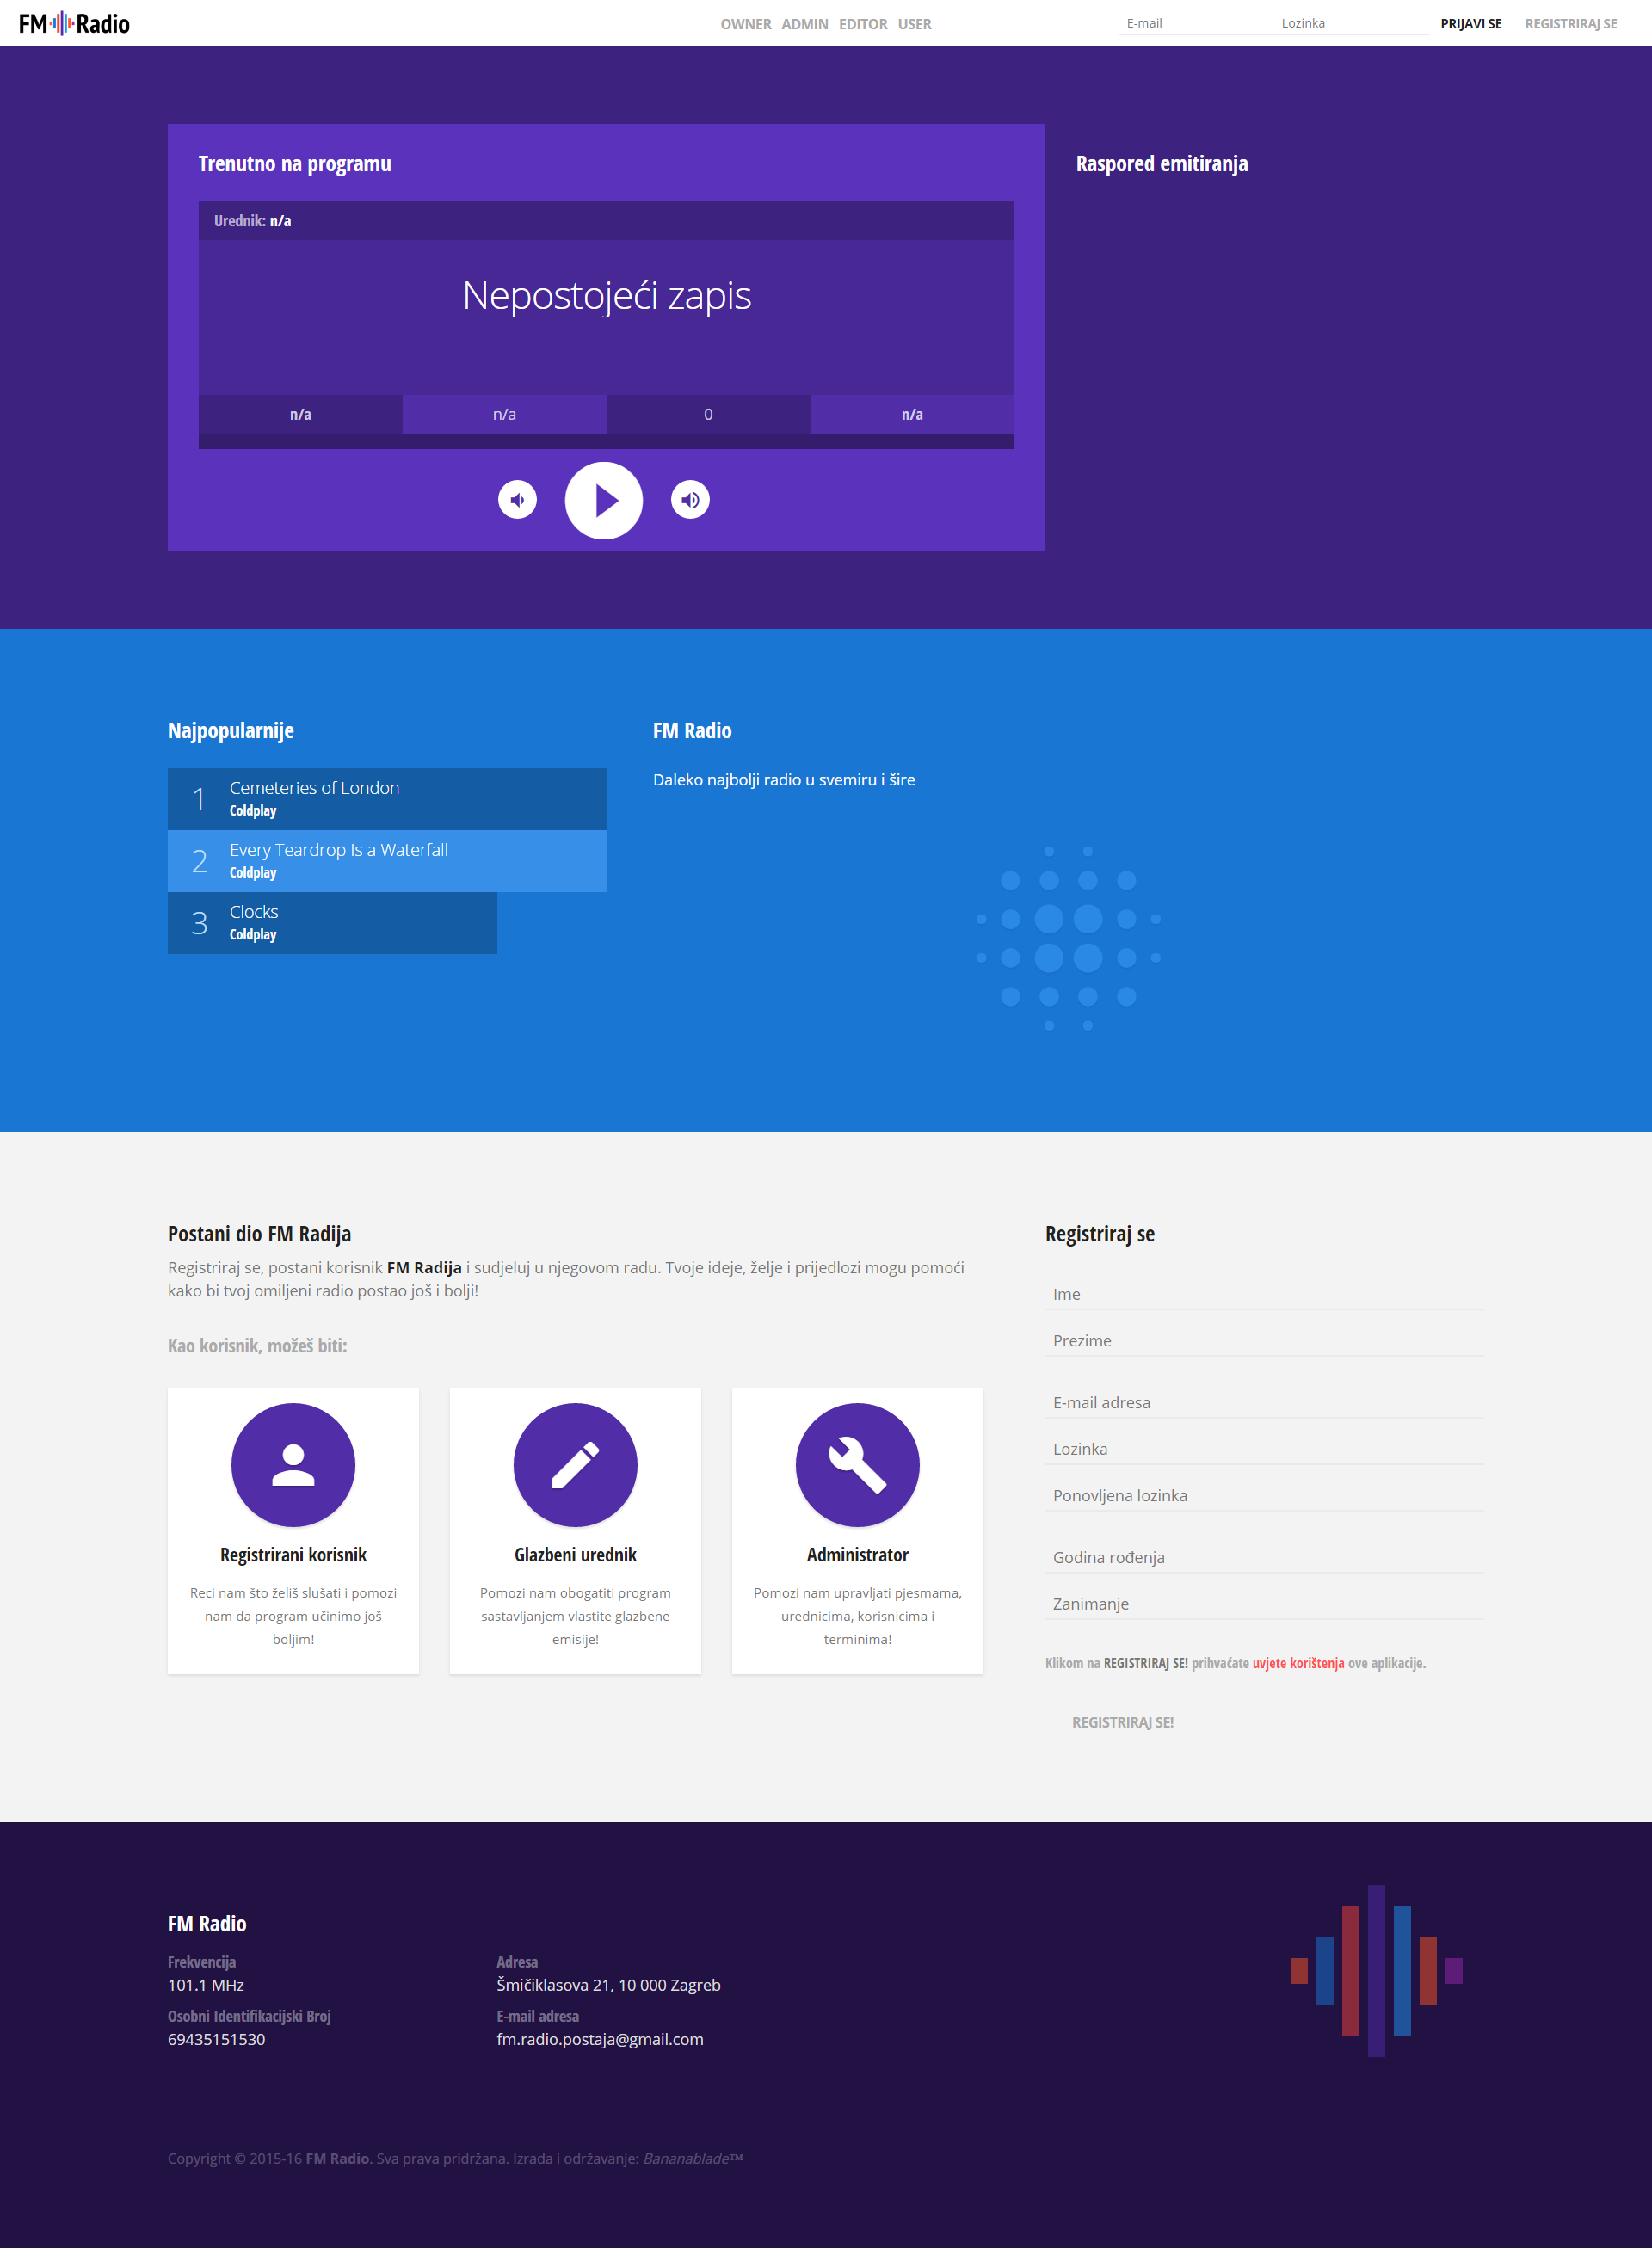
\includegraphics[width=\textwidth]{full_frontpage.png}

\chapter{Zaključak}
Ovaj radi opisuje razvojni proces i implementacijske detalje biblioteke PureScript Angular 2. Na početku su pruženi detalji korištenih tehnologija i standarda koji su korišteni. Glavne tehnologije koje su korištene su jezici PureScript i TypeScript koji se prevode u JavaScript i biblioteka Angular 2. Jezici se izvršavaju na klijentskoj strani je njihova glavna uloga u ovom radu izvršavati kod koji omogućuje korisniku ugodno korištenje korisničkog sučelja svojeg internetskog preglednika. Biblioteka Angular 2 je monolitska biblioteka koja omogućava izradu web sučelja po oblikovnom obrascu model-pogled-model pogleda. Zatim su proučeni problemi i izazovi kod prijenosa biblioteke Angular 2 čija je prva implementacija rađena za objektno orijentirani jezik, a sad radi prijenos u funkcijski deklarativni jezik.

Predstavljeni su uvjeti za izradu minimalnog prihvatljivog proizvoda te je proučeno koji bi bili uvjeti za izradu takvog proizvoda na primjeru prijenosa biblioteke Angular 2 u ekosustav jezika PureScript.

Biblioteka je razvijana proučavanjem koda postojeće web aplikacije za fiktivnu internetsku radijsku postaju FM Radio. Proučavanjem prevedenog koda iz jezika TypeScript u JavaScript se pokušavalo imitirati dobivanje takvog izvršnog koda prevođenjem jezika PureScript. Za postizanje toga se opsežno koristio adaptacijski sloj sučelja stranih funkcija koji je omogućavao ostvarivanje iste funkcionalnosti pozivanjem drugačijih jezičnih konstrukta iz jezika PureScript. U konačnici je osnovna funkcionalnost demonstrirana na primjeru aplikacije internetske radijske postaje uporabom najbitnijih dijelova biblioteke Angular. Prikazan je način na koji se ti jezični konstrukti mogu opisati u jeziku PureScript pomoću razvijane biblioteke.

Potencijalno bi se biblioteku PureScript Angular 2 moglo poboljšavati tako da se na temelju složenije aplikacije prouče algoritmi boljeg prikaza funkcionalnosti izvorne biblioteke. Trenutno postoji samo jedan tip efekta koji opisuje sve efekte koji su posljedica djelovanja aplikacije Angular 2, a PureScript omogućava detaljniju granulaciju istih pa bi se moglo dodatno uvesti podjele na sinkrone i asinkrone efekte, one koji izvode mutacije i one koji ne i slično. Mutacije na dosegu klase bi se mogle grupirati zajedno s pozivima pripadnih funkcija klase u zajedničku monadu te bi se te operacije mogle opisati uporabom sintaksnog šećera (eng. syntactic sugar) koji pružaju kombinatori za monade (eng. monad combinators).

\bibliography{literatura}
\bibliographystyle{fer}

\begin{sazetak}
Pri razvoju Web korisničkih sučelja, sve je više uobičajena uporaba funkcijskog programiranja jer se pogled opisuje deklarativno, a svaka akcija uzrokuje niz ulančanih radnji što se dobro prikazuje u funkcijskim jezicima. U uvodu su opisani detalji korištenih tehnologija, zatim su proučeni problemi i izazovi kod prijenosa biblioteke i na kraju je opisan konkretan primjer implementacije. Ovaj rad opisuje razvojni proces i implementacijske detalje biblioteke PureScript Angular 2. Razvijena biblioteka omogućava korištenje biblioteke Angular 2 u ekosustavu jezika PureScript. Rad se zasniva na primjeni izvorne implementacije biblioteke koja je rađena za objektno orijentirani jezik, a u ovom radu je prenošena u funkcijski deklarativni jezik. 

Proučavanjem prevedenog koda iz jezika TypeScript u JavaScript se pokušavalo imitirati dobivanje takvog izvršnog koda nakon prevođenja iz jezika PureScript. U razvoju se opsežno koristio adaptacijski sloj sučelja stranih funkcija koji je omogućavao ostvarivanje iste funkcionalnosti pozivanjem drugačijih jezičnih konstrukta iz jezika PureScript. U konačnici je osnovna funkcionalnost demonstrirana na primjeru aplikacije internetske radio postaje FM Postaja.

\kljucnerijeci{Funkcijsko programiranje, Web sučelja, Web komponente, PureScript, Angular 2}
\end{sazetak}

\pagebreak
% TODO: Navedite naslov na engleskom jeziku.
\engtitle{Functional approach to Web user interface}
\begin{abstract}
There is a growing trend among frontend developers to use functional programming because the view is described declaratively and every action causes a number of chained events, which can be described accurately with functional languages. Details of the used technologies were described in the prelude, the challenges and obstacles of the process were described after that, and an example of using this library on a real world application was described at the end. This thesis describes the process of developing PureScript Angular 2 library and the details of the implementation. This enables using Angular 2 library inside the PureScript ecosystem. The thesis is based on the original implementation of Angular 2 library which was written in an object oriented language and in this thesis the library was ported to a functional declarative language.

By examining the compiled code from TypeScript language to JavaScript language the goal was to imitate the compiled code from PureScript implementation. To achieve this, an adaptation layer was used which consisted mostly of foreign function interface code which enabled achieving the same functionality by calling different language constructs from the language PureScript. At the end, the basic functionality was demonstrated on an example of web application for an internet radio station FM Postaja.

\keywords{Functional programming, Web interfaces, Web components, PureScript, Angular 2}
\end{abstract}

\pagebreak
\section*{Dodatak A: Sadržaj priloženog medija (CD/DVD)}
Na priloženom mediju se nalaze svi materijali korišteni za izradu ovog rada. 


\begin{center}
    \begin{tabular}{ | l | l | p{9cm} |}
    \hline
    R.br. & Mapa/Datoteka & Sadržaj \\ \hline
    
    1. & PROCITAJ\_ME.TXT & Informacije o sadržaju medija \\ \hline
    
    2. & /tex & Tekst rada u izvornom formatu (LaTex) i pripadne datoteke \\ \hline
    
    3. & /Ivosevic\_Funkcijski\_pristup.pdf & Tekst rada u pdf formatu \\ \hline
    4. & /Ivosevic\_Funkcijski\_pristup.ppt & Prezentacija \\ \hline
    
    5. & /izvorni\_kod & Izvorni kod izrađene biblioteke s uputama za korištenje \\ \hline
    
    \end{tabular}
\end{center}


\end{document}
